
\chapter{Introducción}
\label{chap:introduccion} 
Este Trabajo Fin de Grado se enmarca en el ámbito educativo, en concreto en la "Gamificación de una plataforma educativa". Según avanza la ciencia y la tecnología la sociedad ha cambiado y las formas de enseñar también. Este proyecto tiene como objetivo crear nuevos juegos y ejercicios que permitan enseñar a programar a los más jóvenes de una forma más divertida para fomentar el aprendizaje y la motivación, así como mejorar sus habilidades. Este proyecto engloba cuantiosas tecnologías web y herramientas que han servido para crear nuevos ejercicios para la plataforma de Robótica educativa \textit{Kibotics} de la Asociación de Robótica e Inteligencia Artificial \textit{JdeRobot}.

En este capítulo se hace una breve introducción del uso actual de la Robótica y las tecnologías web, conceptos clave para ponernos en contexto y enfatizar en el tema principal de este trabajo: la 'Gamificación'.


%%%%%%%%%%%%%%%%%%%%%%%%%%%%%%%%%%%%%%%%%%%%%%%%%%%%%%%%%%%%%%%%%%%%%%%%%%%%%%%%%%%%%%%%%%%%%%%%%%%%%%%%%%%%%%%%
\section{Robótica}\label{motivacion}
La Robótica es una rama de la ingeniería que combina diversas áreas de conocimiento como son las matemáticas, la electrónica, mecánica, informática y física. \\

A lo largo de la historia el ser humano siempre ha tenido interés en recrear partes del ser humano con el uso de máquinas para facilitarse la vida o bien para comprenderla. No fue hasta el siglo XVIII con  la Revolución Industrial cuando se impulsó la posible realización de estos pensamientos. 

El término \textit{robot} proviene del vocablo checo \textit{robota}, que significa servidumbre o trabajo esclavizador. Fue usado por primera vez por el dramaturgo checoslovaco Karel Capek(1890-1938) en su obra de teatro: Rossum´s Universal Robots, en 1920, una obra teatral basada en la ciencia ficción donde se construyen humanos artificiales para que realicen trabajos forzosos. \footnote{https://www.muyinteresante.es/cultura/arte-cultura/articulo/iquien-invento-la-palabra-robot#:~:text=Robot%20es%20un%20t%C3%A9rmino%20que,su%20obra%20de%20teatro%20Rossum%3F 
}
\\\\
No fue hasta los años 50 cuando se desarrollaron los primeros robots.
Actualmente con el rápido avance en tecnológia la realidad ha superado a la ficción, estamos rodeados de robots. La Figura 1.1 muestra algunos ejemplos y aunque parezcan muy diferentes, tienen muchas cosas en común.
\\
\begin{figure}[h]
  \begin{subfigure}[b]{0.25\textwidth}
    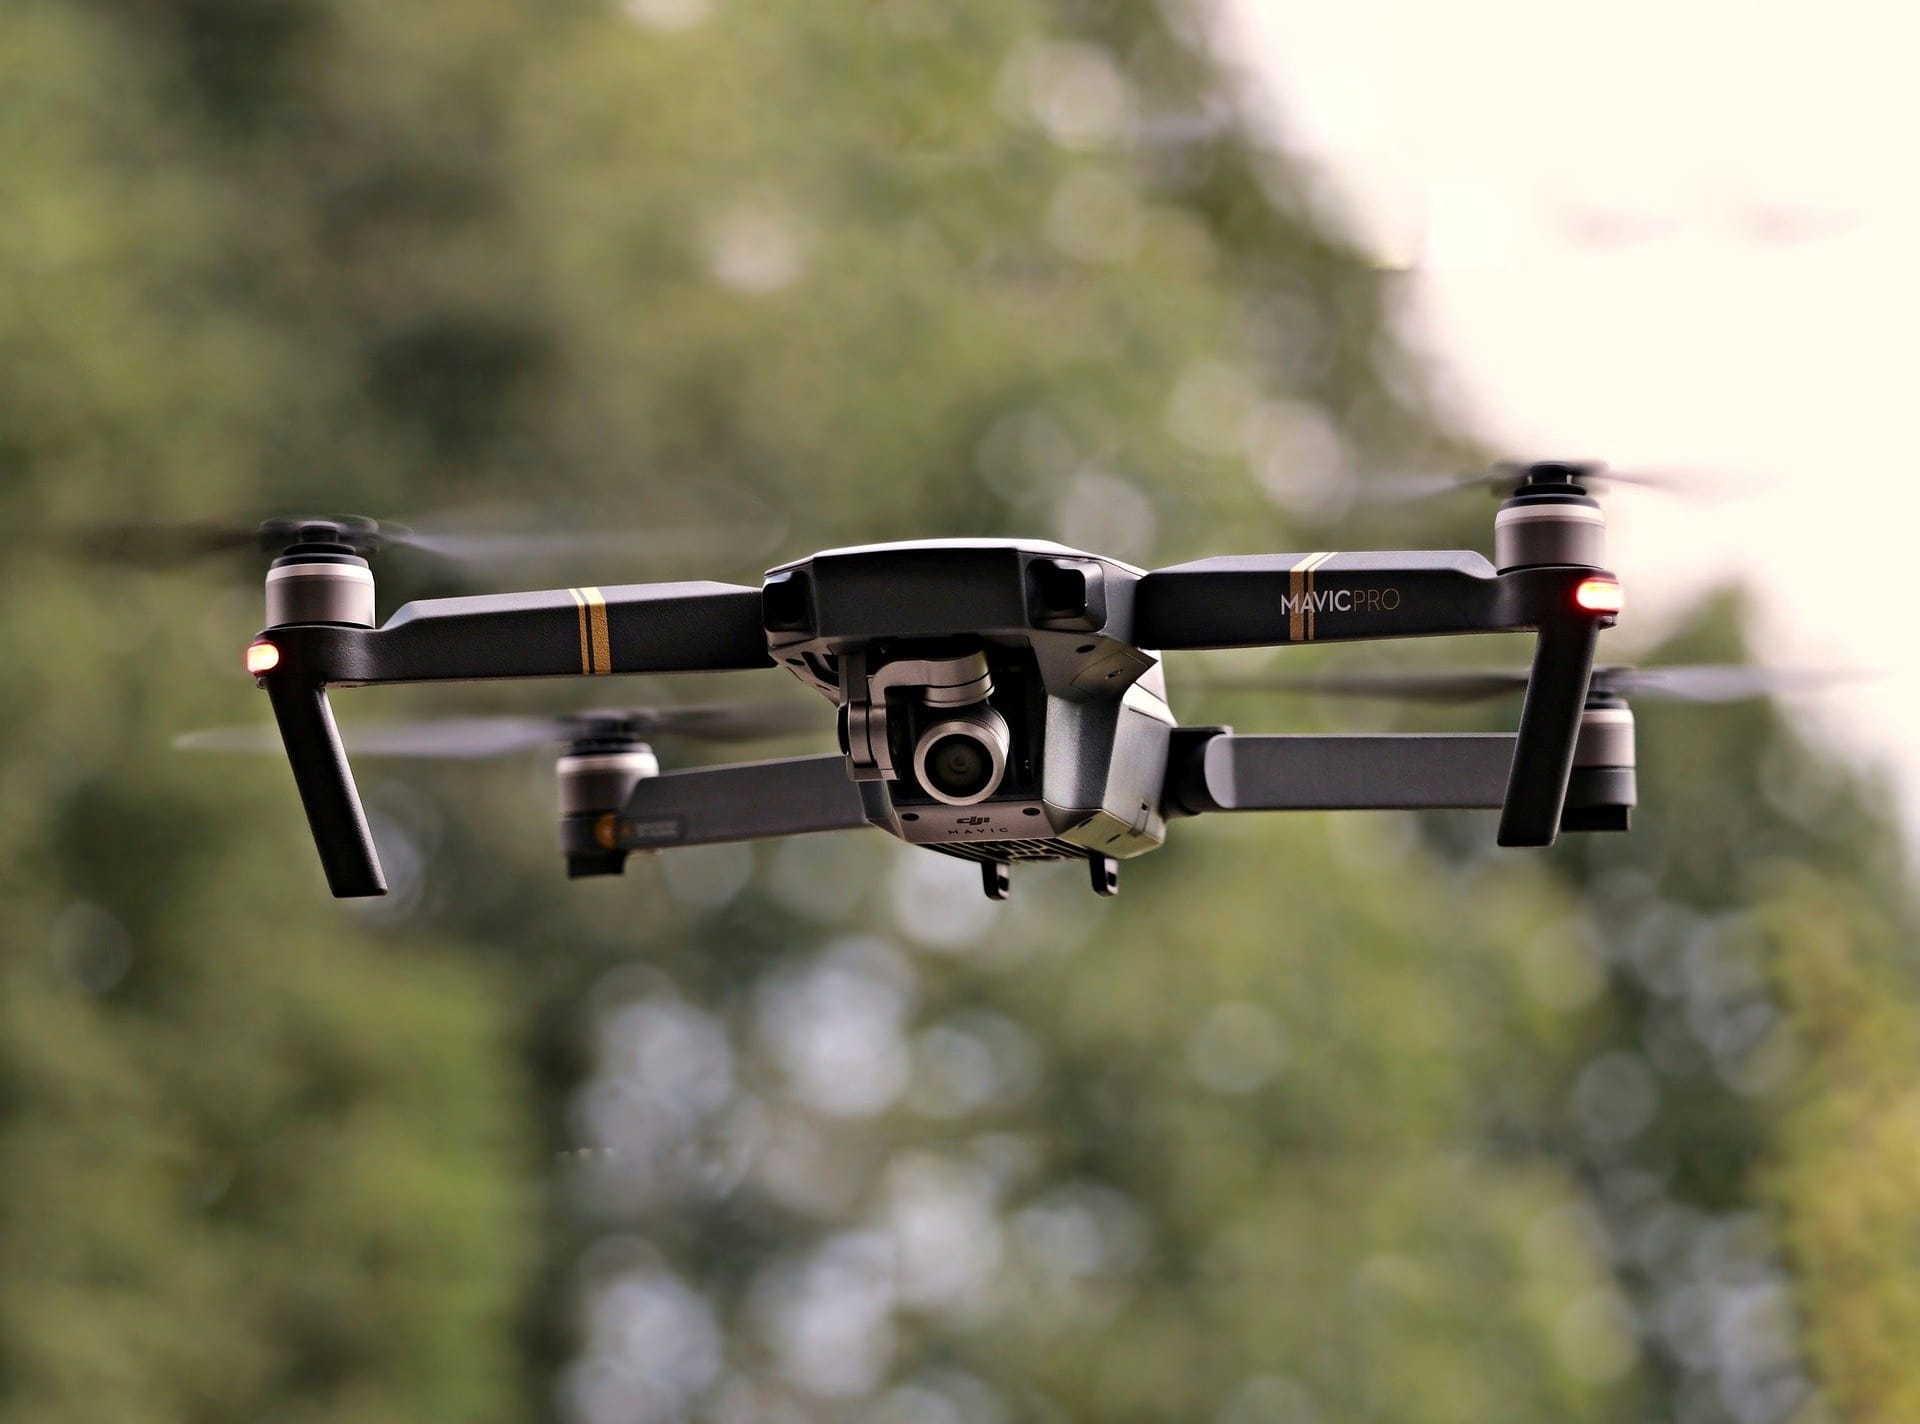
\includegraphics[width=\textwidth, height=\textwidth]{chapters/images/drone.jpeg}
    \caption{Drone}
    \label{fig:f1}
  \end{subfigure}
  \hfill
  \begin{subfigure}[b]{0.25\textwidth}
    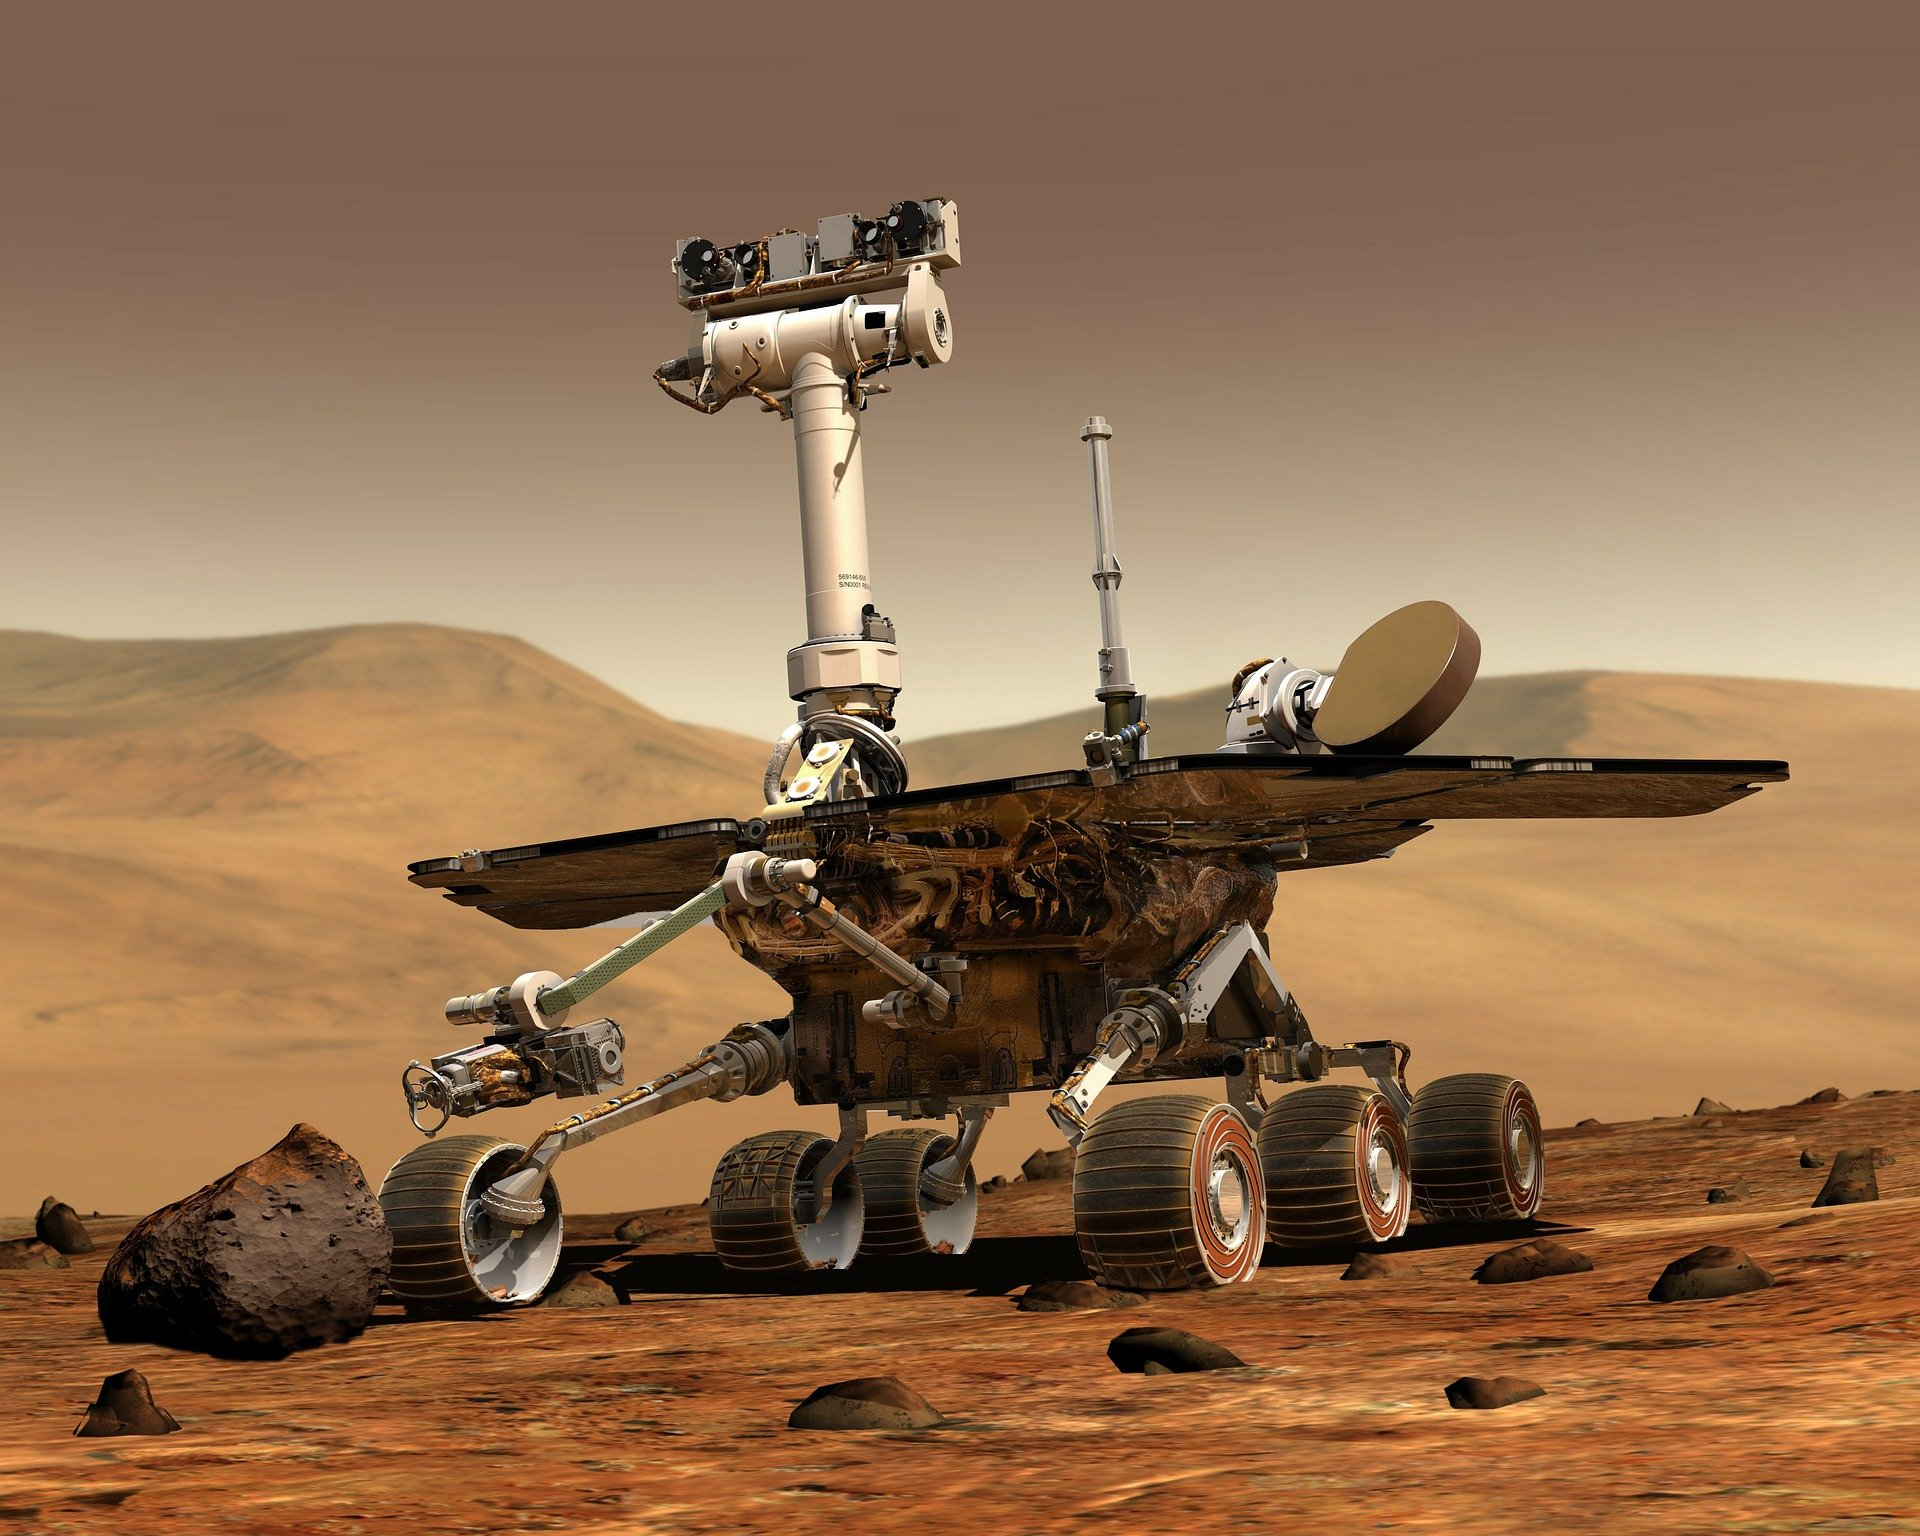
\includegraphics[width=\textwidth, height=\textwidth]{chapters/images/mars.jpg}
    \caption{Perseverance Mars}
    \label{fig:f2}
  \end{subfigure}
  \hfill
   \begin{subfigure}[b]{0.25\textwidth}
    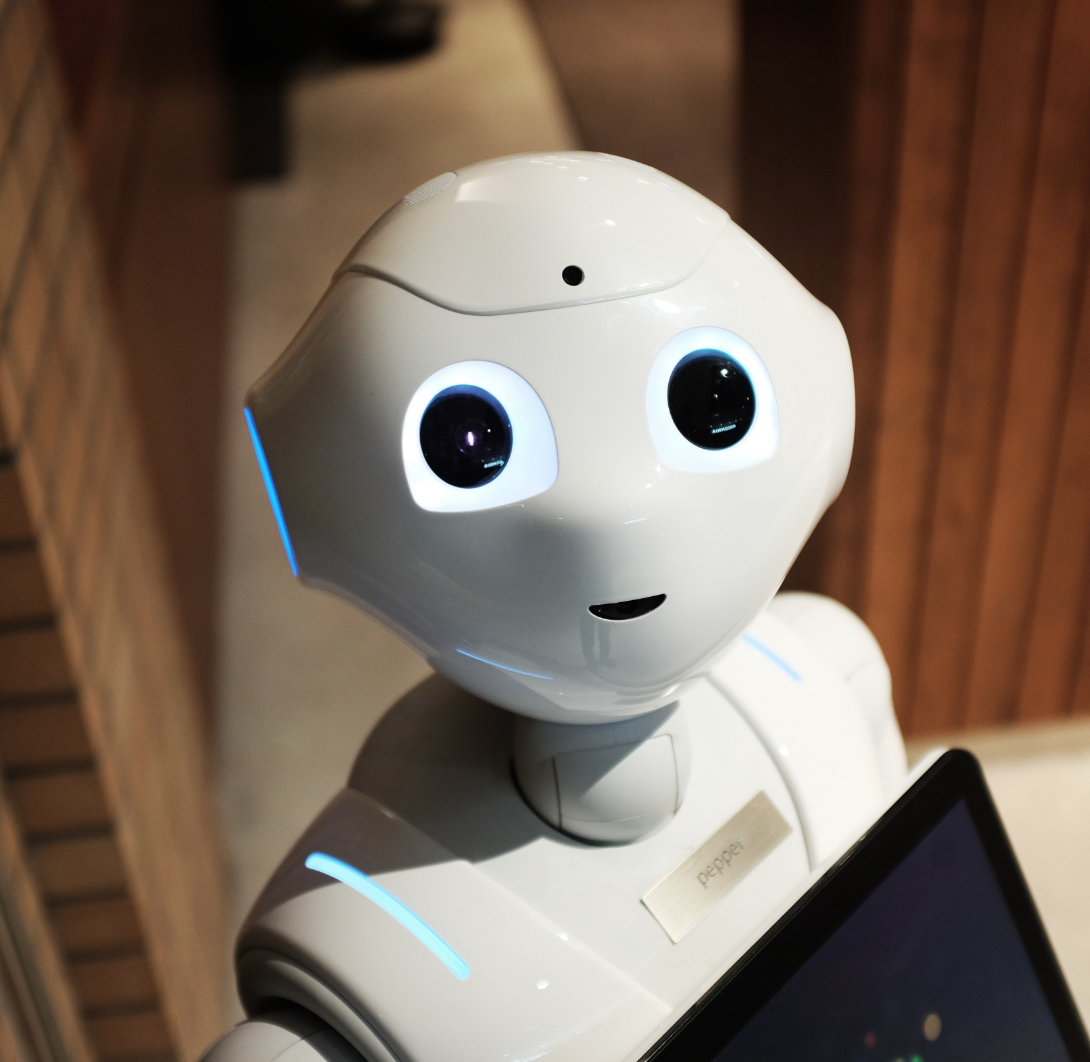
\includegraphics[width=\textwidth, height=\textwidth]{chapters/images/nao.png}
    \caption{Nao}
    \label{fig:f3}
  \end{subfigure}
  \hfill
   \begin{subfigure}[b]{0.25\textwidth}
    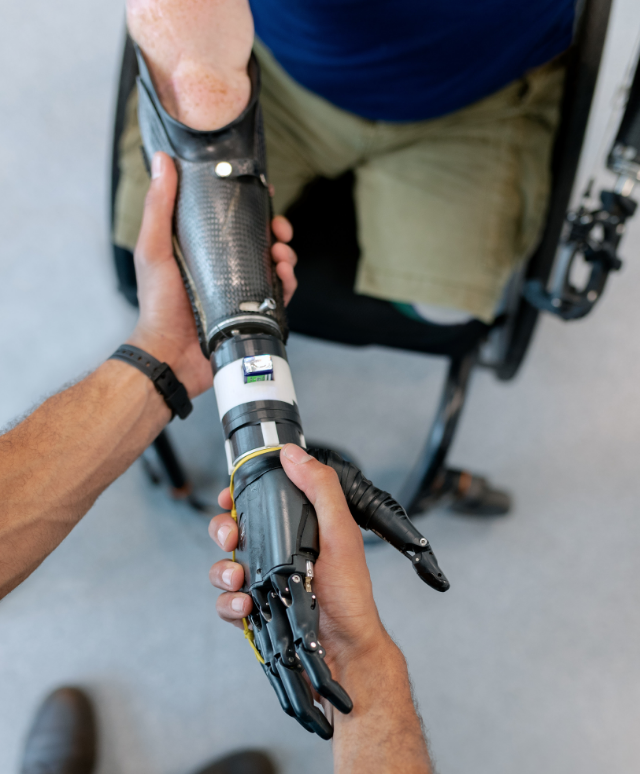
\includegraphics[width=\textwidth, height=\textwidth]{chapters/images/brazo.png}
    \caption{Brazo biónico}
    \label{fig:f4}
  \end{subfigure}
  \hfill
   \begin{subfigure}[b]{0.25\textwidth}
    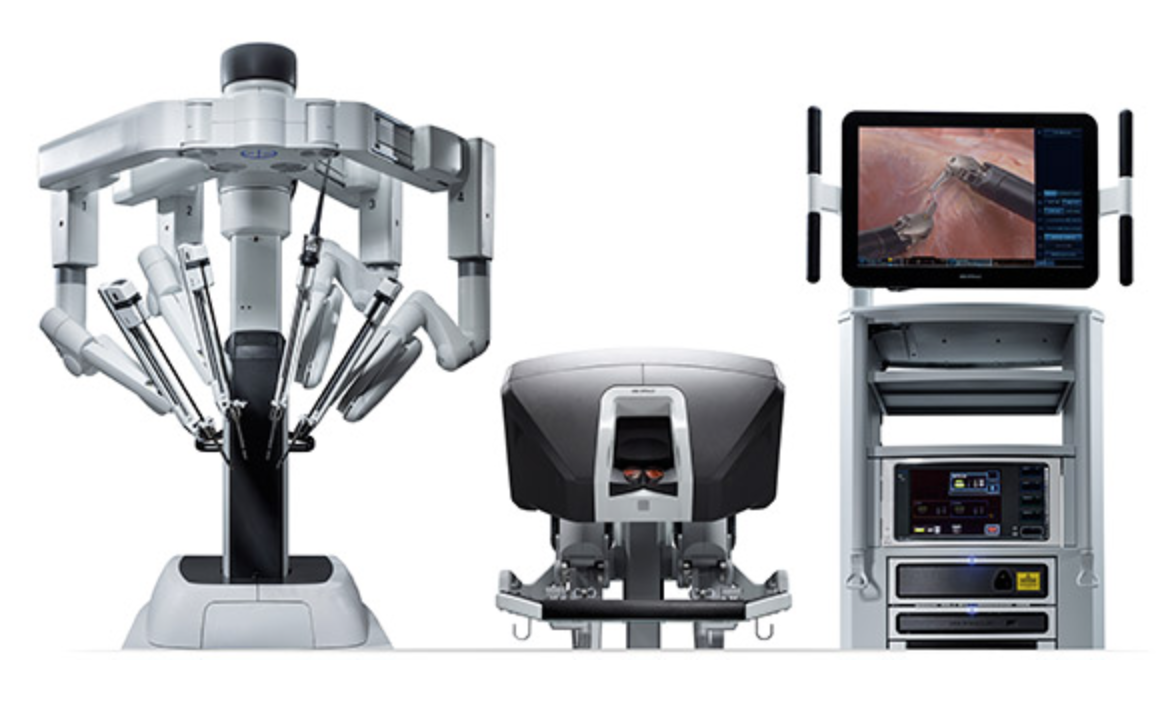
\includegraphics[width=\textwidth, height=\textwidth]{chapters/images/davinci.png}
    \caption{Da Vinci }
    \label{fig:f5}
  \end{subfigure}
  \hfill
   \begin{subfigure}[b]{0.25\textwidth}
    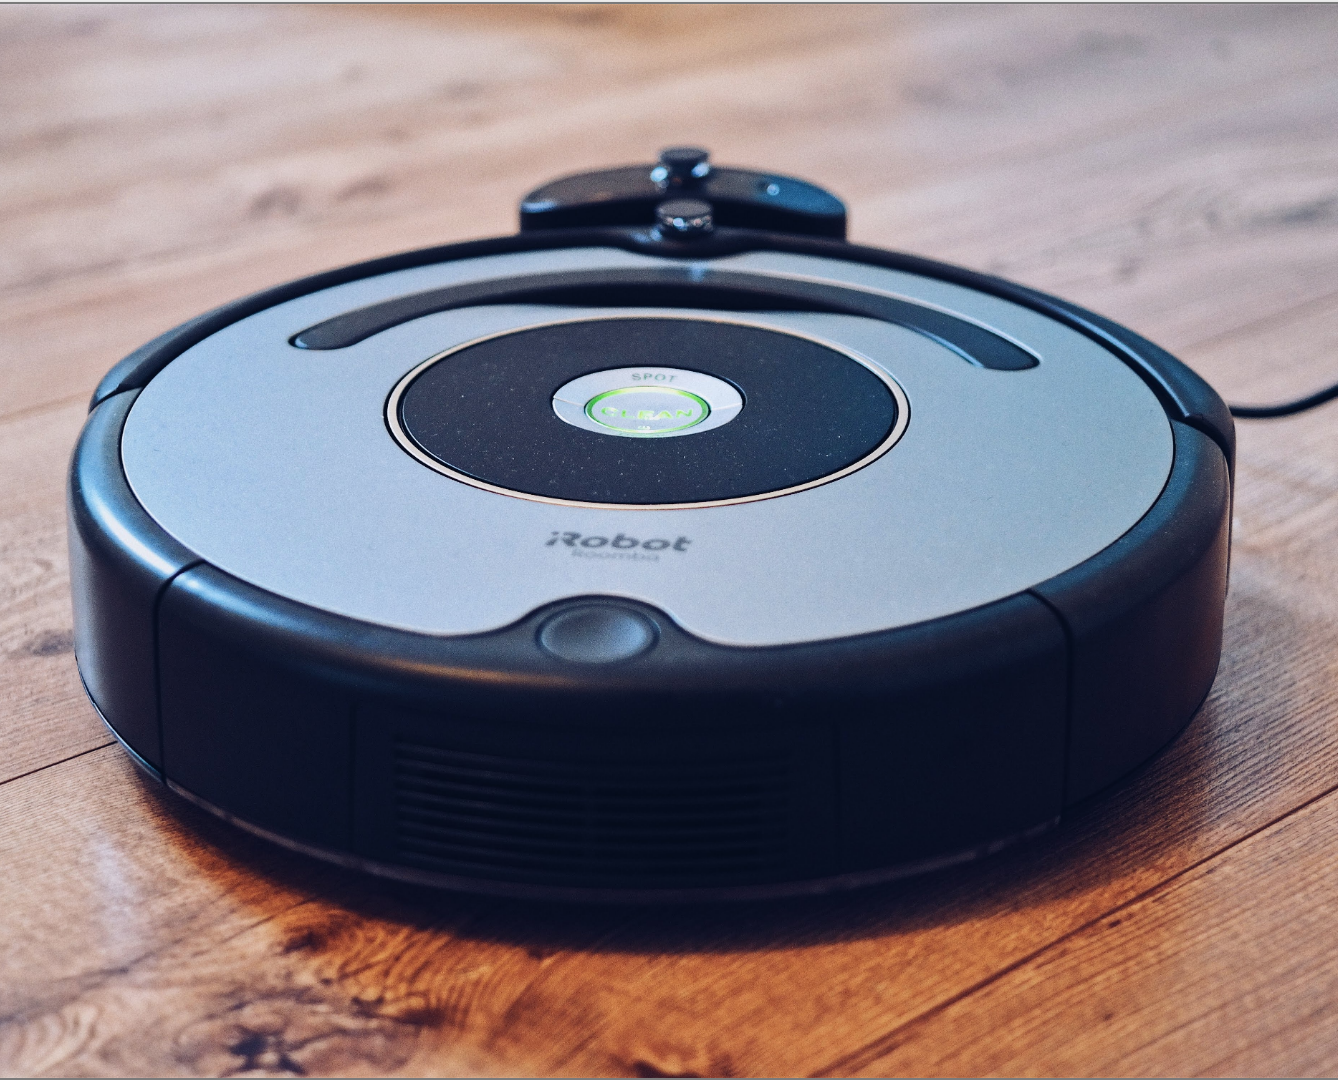
\includegraphics[width=\textwidth, height=\textwidth]{chapters/images/roomba.png}
    \caption{Roomba}
    \label{fig:f6}
  \end{subfigure}
  \caption{Ejemplos de Robots}
\end{figure}

Bajo el nombre robot agrupamos máquinas muy distintas desde robots de limpieza o cocina, robots de las fábricas, incluso robots que salvan vidas. Es por esto que para diferenciarlos se dividen según el entorno de aplicación, robots industriales (brazos y pinzas para ensamblado de piezas) y robots de servicio (destinados a limpieza, coches autónomos, investigación en terrenos hostiles o fines medicos). También se pueden clasificar por su forma (los Androides y zoomórficos), si son fijos o móviles, terrestres, acuáticos o áereos. \\Vamos a ver qué tienen en común todos estos robots.
Un robot es una máquina autónoma que es capaz de percibir su entorno , realizar ciertos cálculos para tomar decisiones, actuar en el mundo real de acuerdo con esas decisiones y comunicarse con otras máquinas o con humanos.
Para todo ello utilizan:


\begin{itemize}
  \item Sensores: para recibir información de su entorno (láser, lídar ultrasonidos, infrarrojos, cámaras, radio frecuencia, sensores térmicos...). Ver Figura 1.2.a
  \item Actuadores:  permiten la locomoción del robot por su entorno y manipulación de objetos (Motores eléctricos, de combustión, amortiguadores, hélices, patas, ruedas, cadenas...). Ver Figura 1.2.c
  \item Procesador y algoritmos: para el cálculo y toma de decisiones. Ver Figura 1.2.b
  \item Leds, Pantallas, Antenas, Altavoces...: para comunicarse con otros robots o con humanos. Ver Figura 1.2.d
\end{itemize}

\begin{figure}[h]
\begin{subfigure}{.5\textwidth}
  \centering
  % include first image
  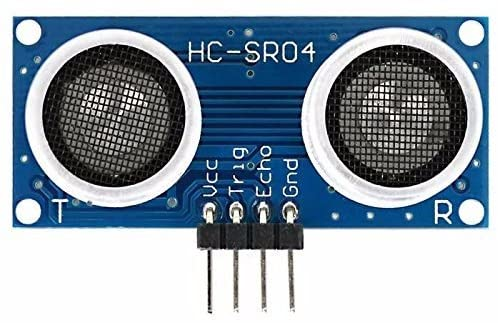
\includegraphics[width=.6\linewidth]{chapters/images/us.jpg}  
  \caption{Sensor ultrasonidos}
  \label{fig:sub-first}
\end{subfigure}
\begin{subfigure}{.5\textwidth}
  \centering
  % include second image
  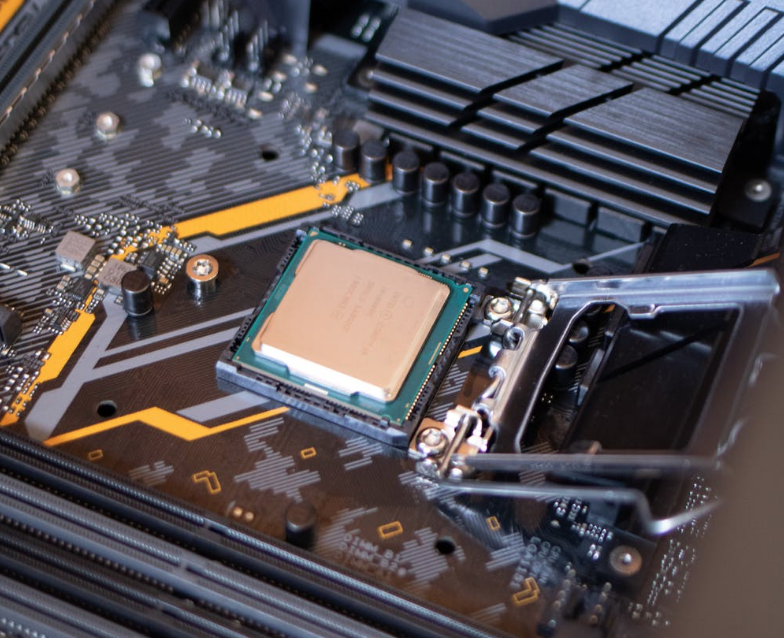
\includegraphics[width=.6\linewidth]{chapters/images/procesador.png}  
  \caption{Procesador}
  \label{fig:sub-second}
\end{subfigure}


\begin{subfigure}{.5\textwidth}
  \centering
  % include third image
  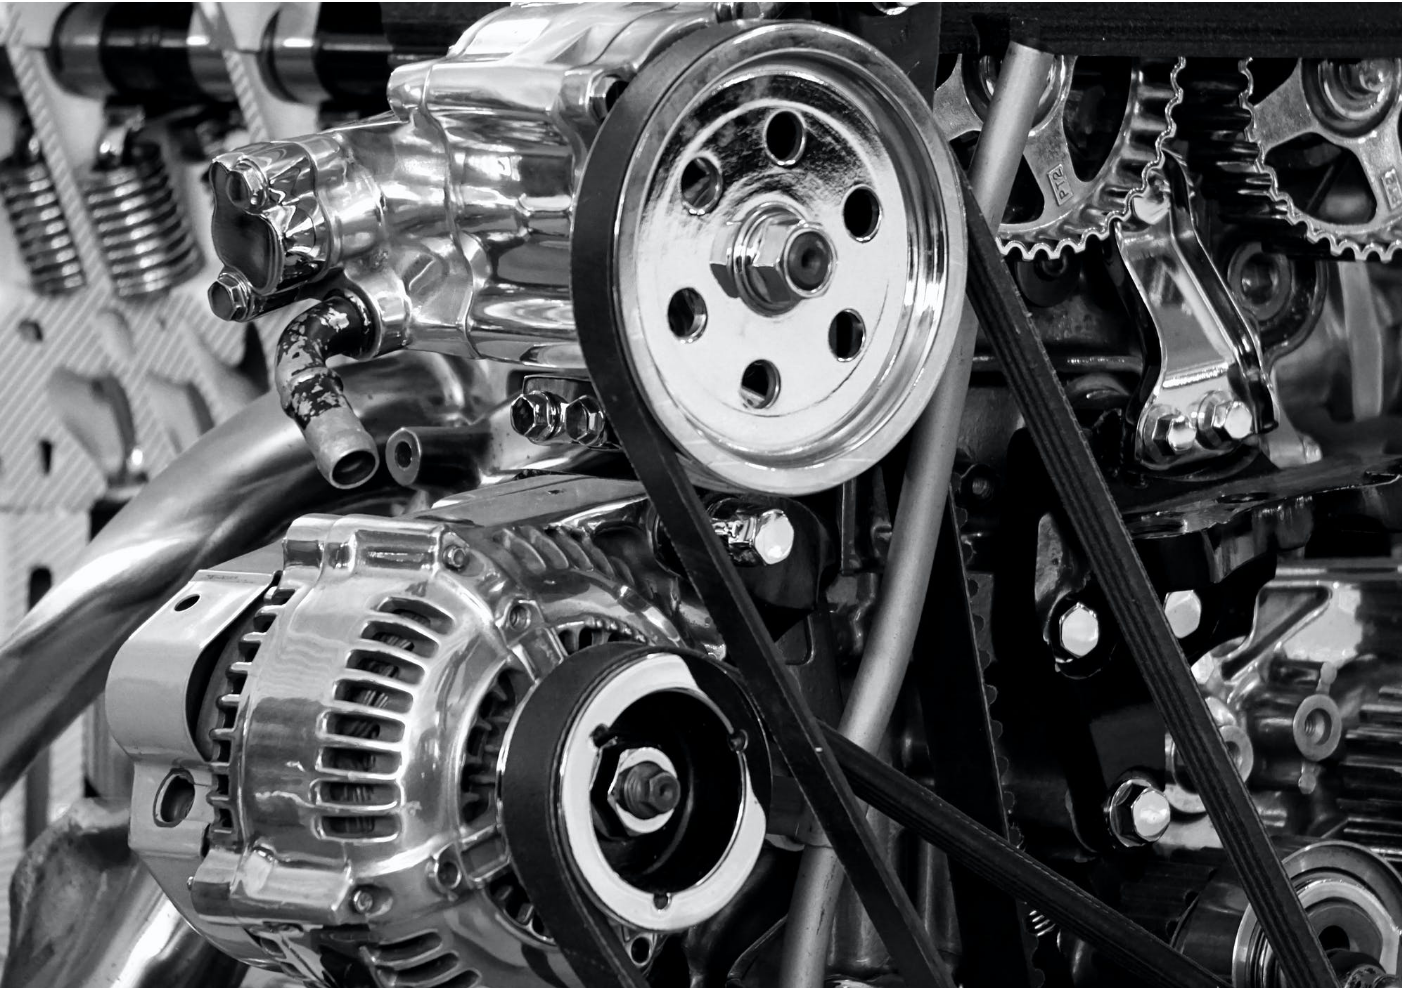
\includegraphics[width=.6\linewidth]{chapters/images/motor.png}  
  \caption{Motor}
  \label{fig:sub-third}
\end{subfigure}
\begin{subfigure}{.5\textwidth}
  \centering
  % include fourth image
  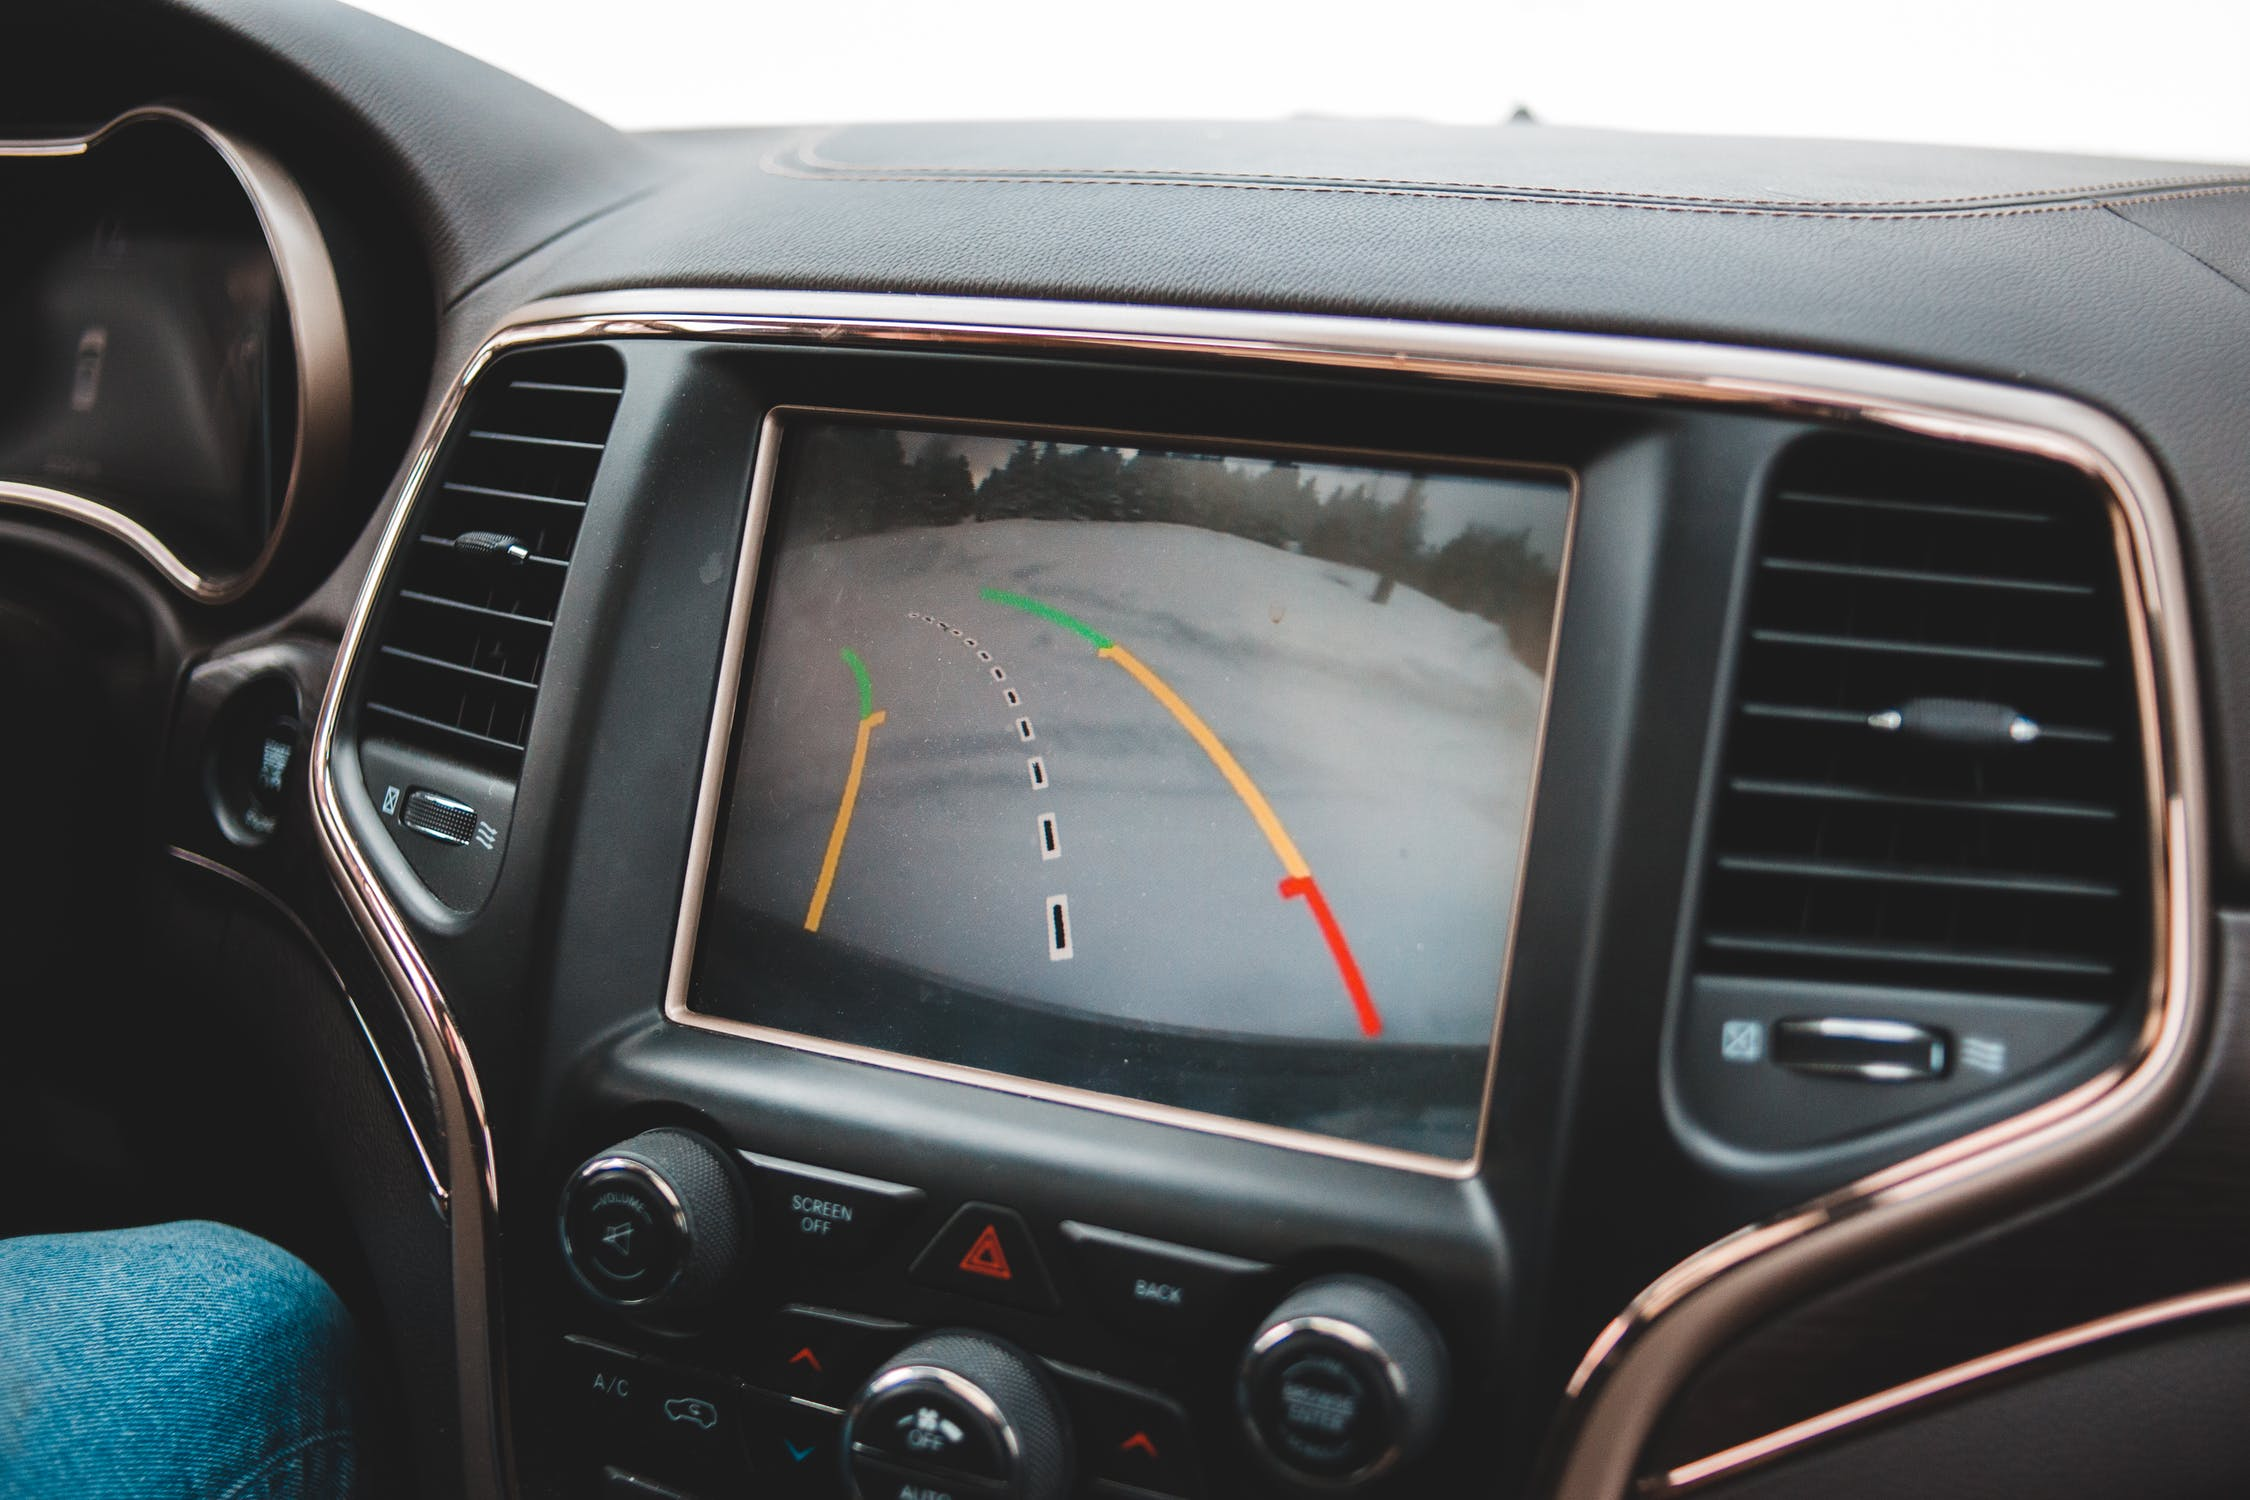
\includegraphics[width=.6\linewidth]{chapters/images/pantalla.jpeg}  
  \caption{Pantalla}
  \label{fig:sub-fourth}
\end{subfigure}
\caption{Ejemplos partes de un robot}
\label{fig:partes robot}
\end{figure}

Recientemente la robótica se está imporporando a las aulas para que los más pequeños adquieran conocimientos y habilidades muy importantes para su futuro, en la siguiente Figura 1.3 se muestran unos ejemplos de Robots diseñados para el ámbito educativo.

\begin{figure}
 \centering
  \subfloat[Bee-bot]{
   \label{f:beebot}
    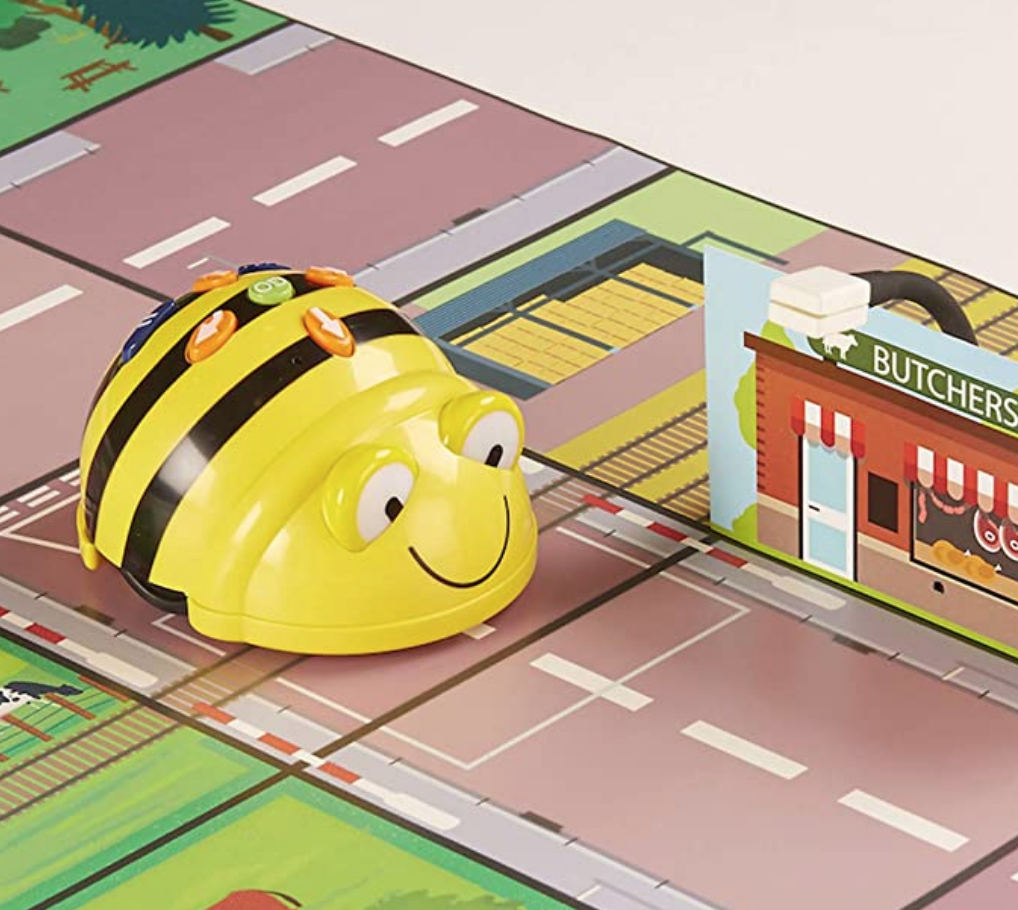
\includegraphics[width=0.3\textwidth]{chapters/images/beebot.png}}
  \subfloat[Makeblock Mbot]{
   \label{f:mbot}
    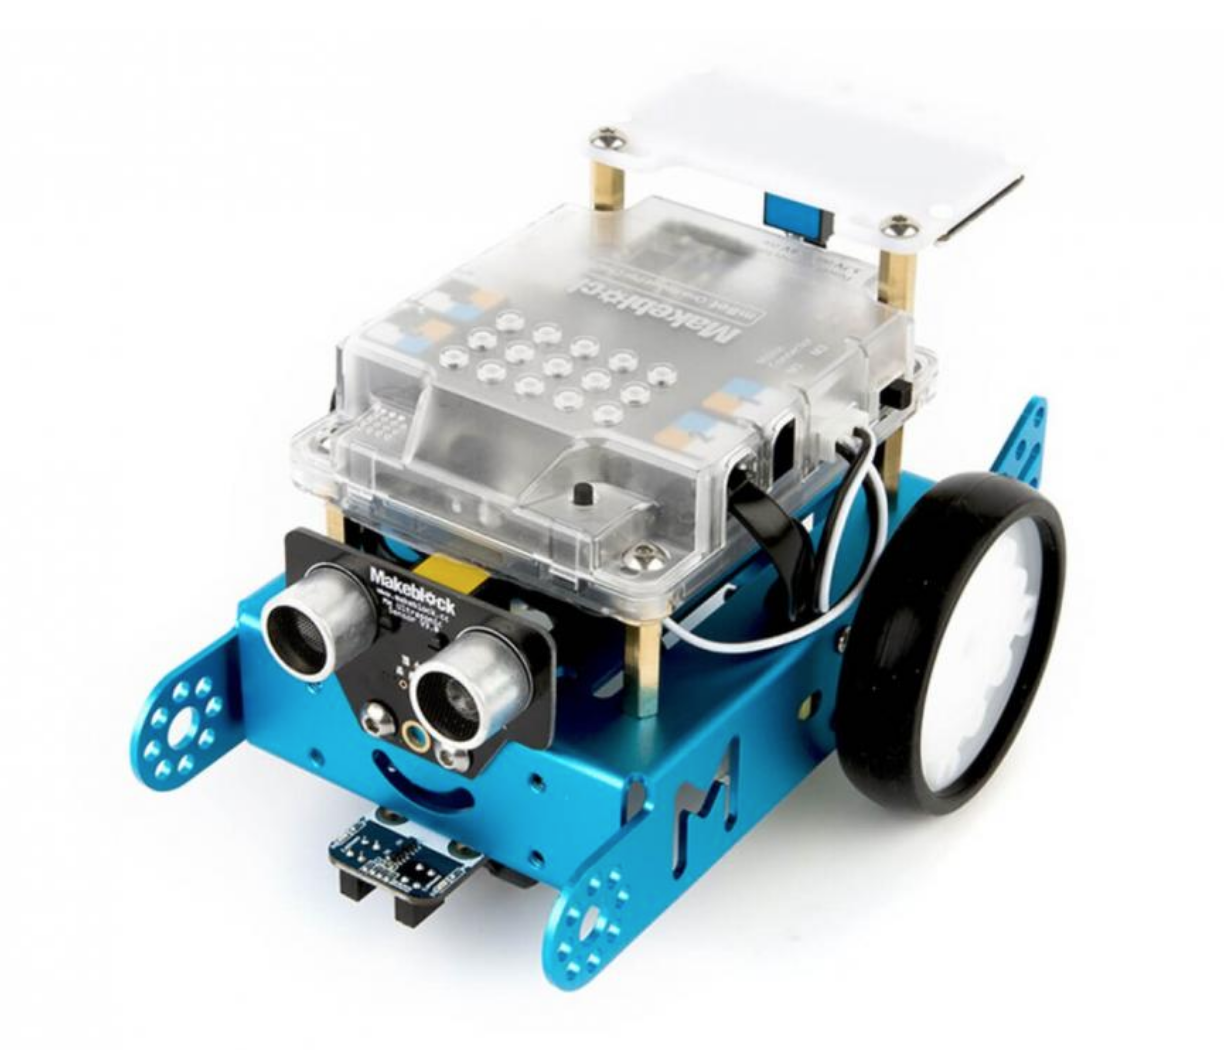
\includegraphics[width=0.3\textwidth]{chapters/images/mbot.png}}
  \subfloat[LEGO MINDSTORMS EV3 ]{
   \label{f:legomindstorms}
    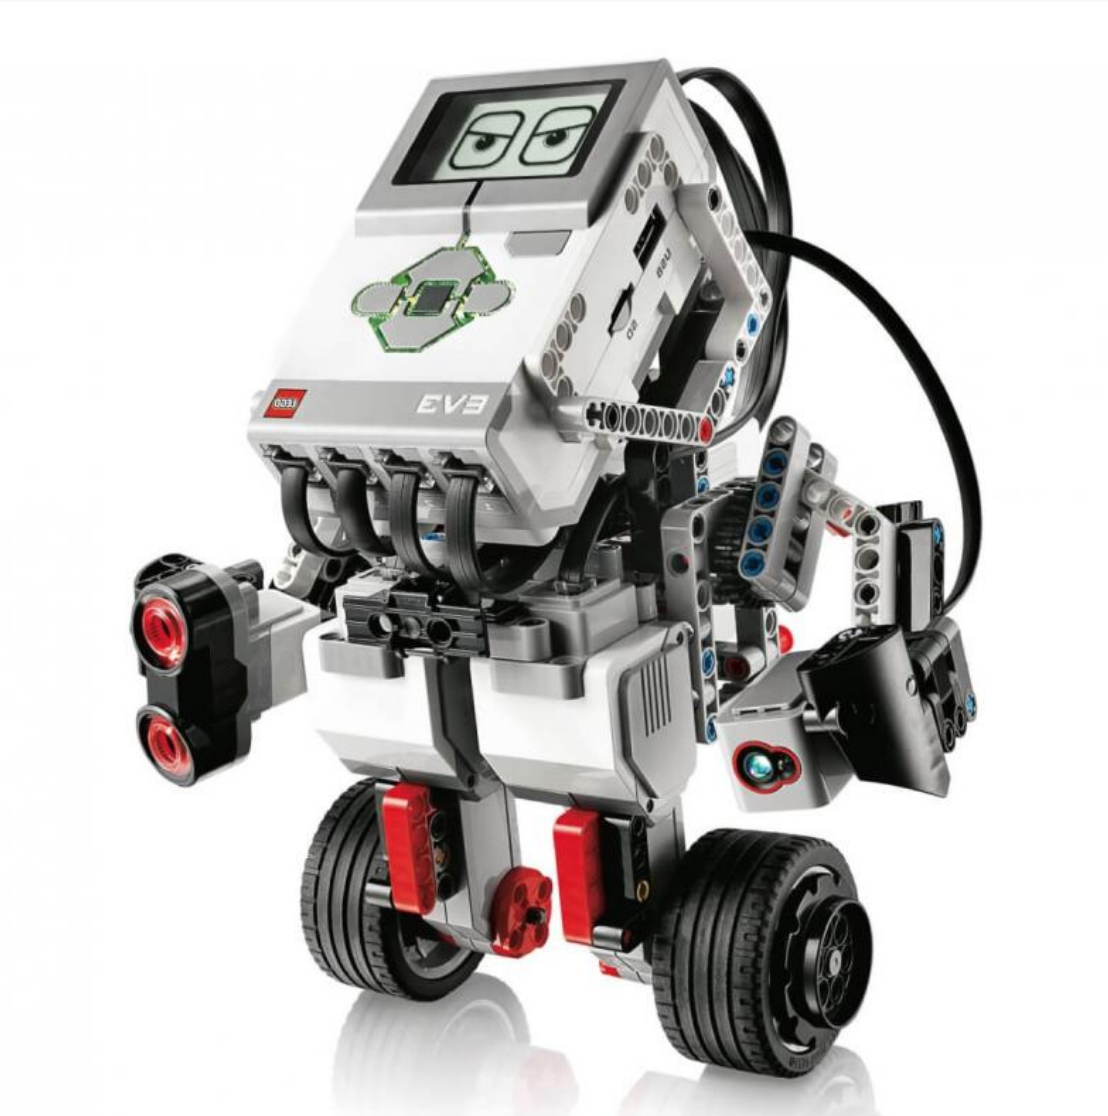
\includegraphics[width=0.3\textwidth]{chapters/images/lego.png}}
 \caption{Ejemplos de Robots educativos}
 \label{f:robotseducativos}
\end{figure}


%%%%%%%%%%%%%%%%%%%%%%%%%
\section{Tecnologías Web}
Las tecnologías web juegan un papel muy importante en el mundo moderno gracias a Internet. Esta plataforma WWW(World Wide Web) 
ha ido evolucionado hasta poder implementar potentes aplicaciones con un modelo cliente/servidor. En la siguiente Figura 1.4 podemos ver algunos ejemplos de aplicaciones web.

\begin{figure}[h]
\begin{subfigure}{.5\textwidth}
  \centering
  % include first image
  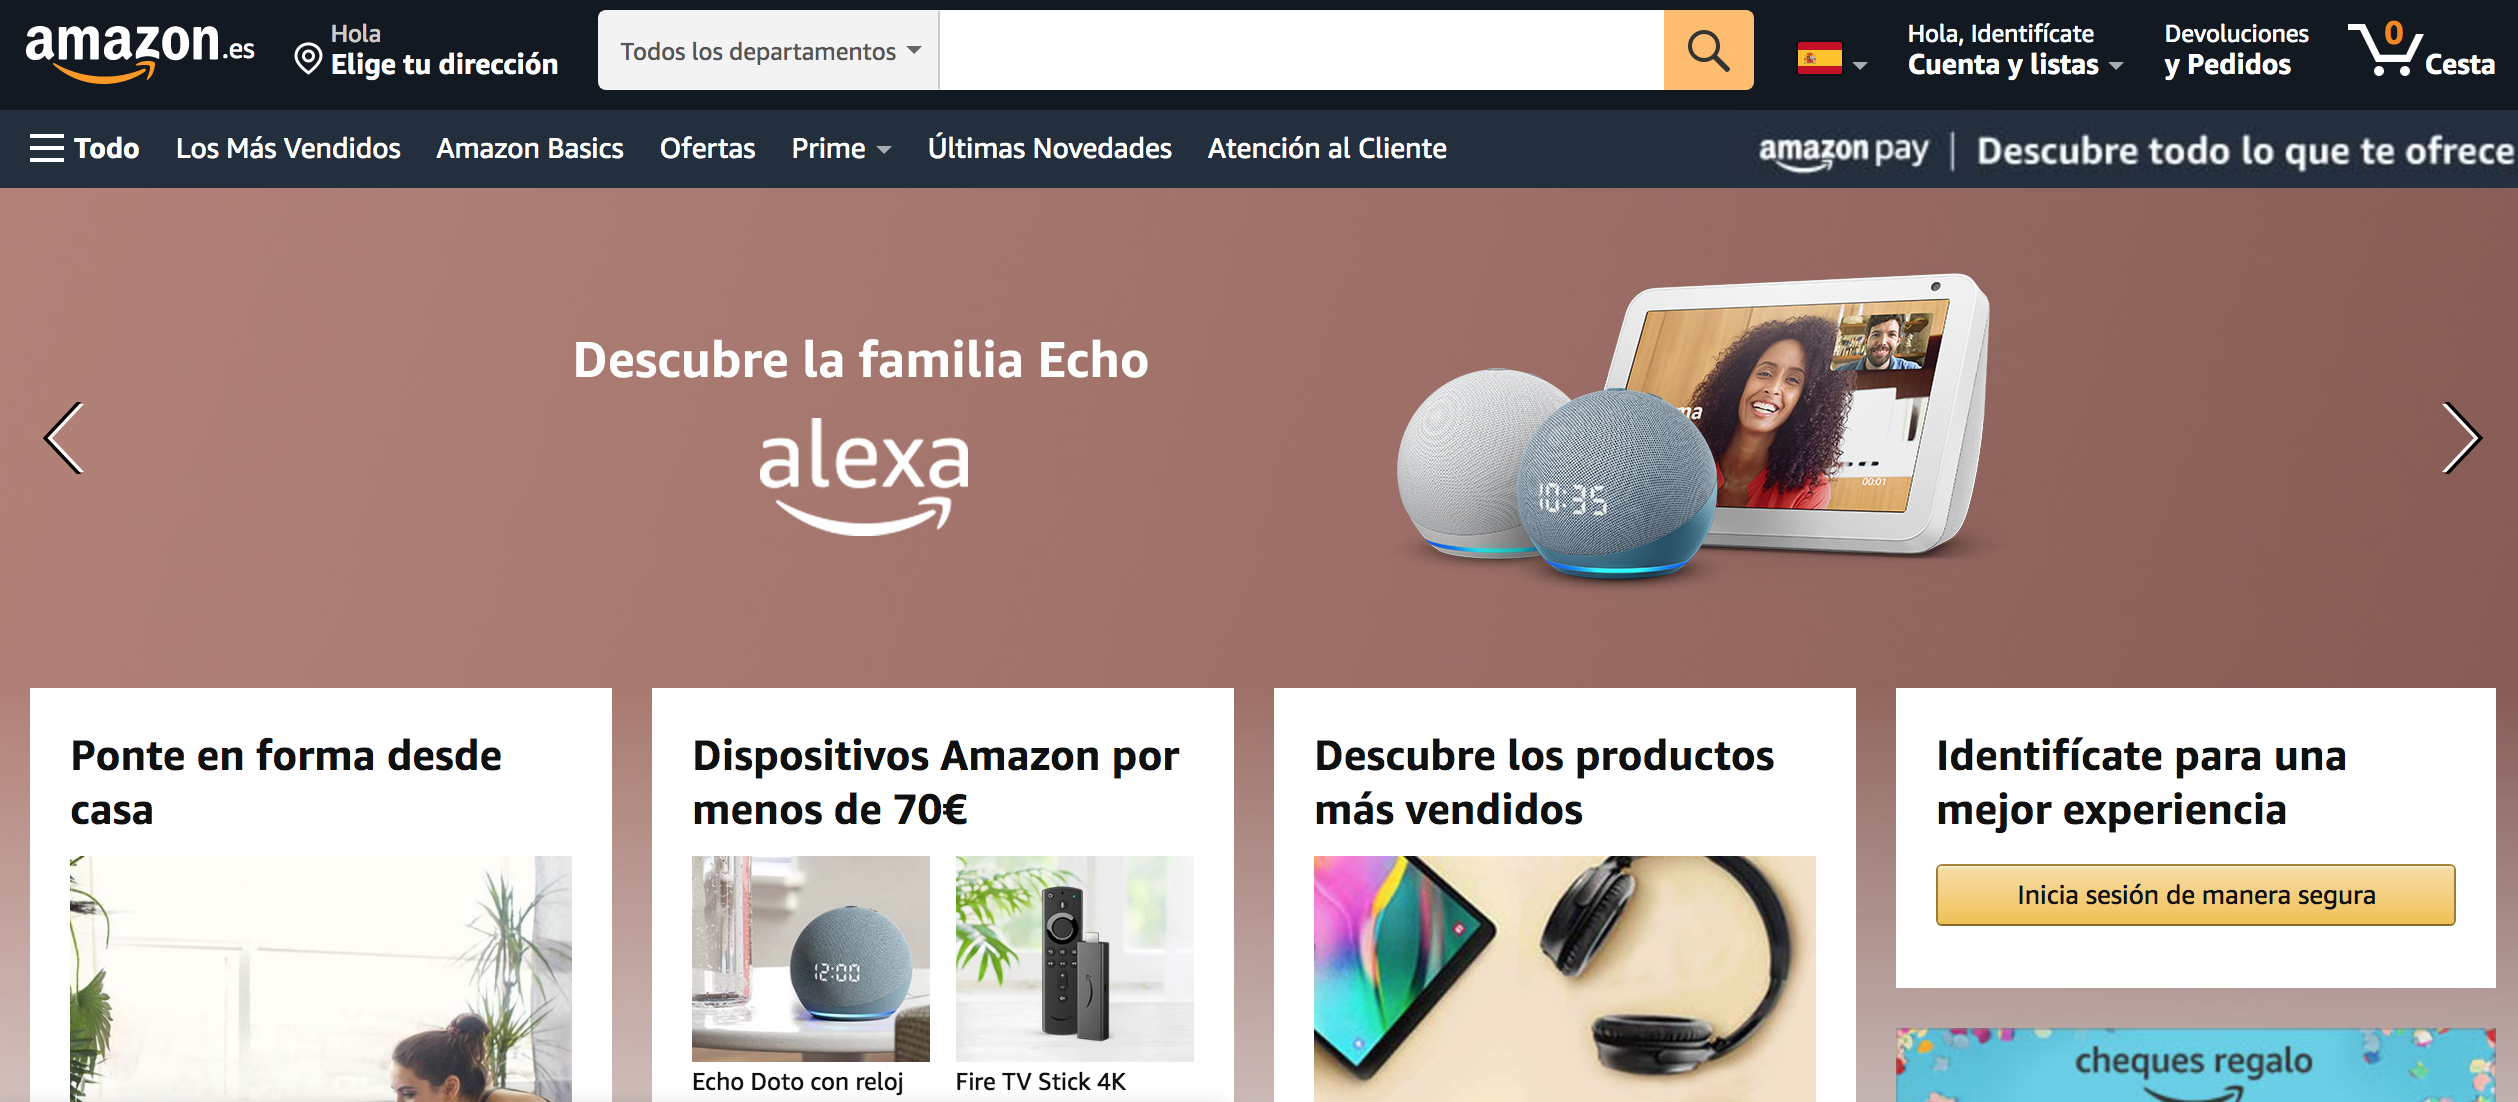
\includegraphics[width=.6\linewidth]{chapters/images/amazon.png}  
  \caption{Amazon}
  \label{fig:sub-first}
\end{subfigure}
\begin{subfigure}{.5\textwidth}
  \centering
  % include second image
  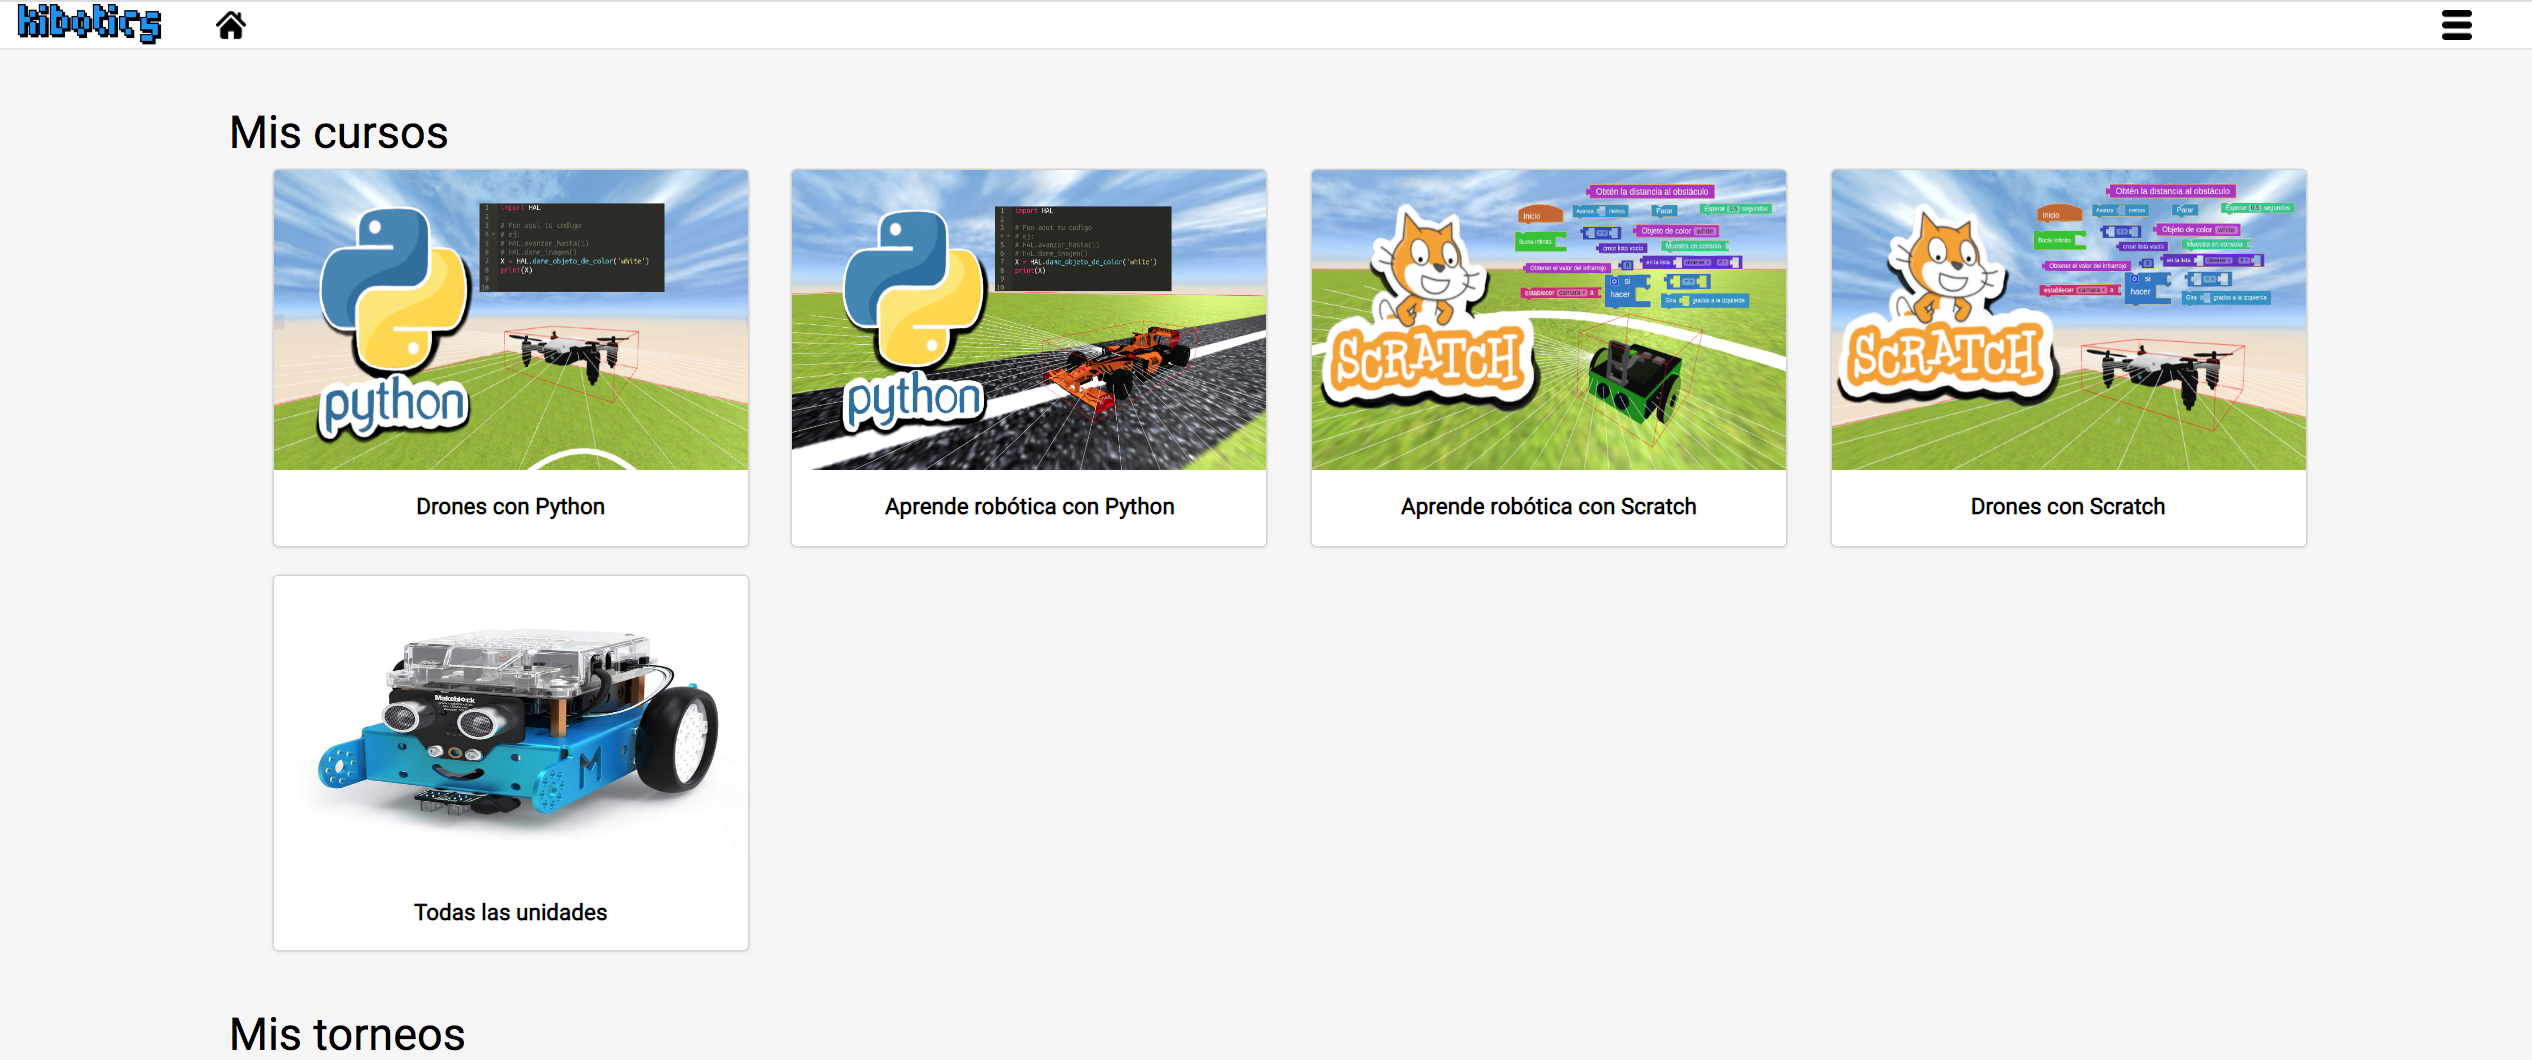
\includegraphics[width=.6\linewidth]{chapters/images/kibotics.png}  
  \caption{Kibotics}
  \label{fig:sub-second}
\end{subfigure}
\begin{subfigure}{.5\textwidth}
  \centering
  % include third image
  
\includegraphics[width=.6\linewidth]{chapters/images/disney.jpeg}  
  \caption{Disney+}
  \label{fig:sub-third}
\end{subfigure}
\begin{subfigure}{.5\textwidth}
  \centering
  % include fourth image
  
\includegraphics[width=.6\linewidth]{chapters/images/urjcweb.png}  
  \caption{URJC}
  \label{fig:sub-fourth}
\end{subfigure}
\caption{Ejemplos aplicaciones web}
\label{fig:partes robot}
\end{figure}

La web es una colección de documentos enlazados a través de hiperenlaces, cada recurso queda definido por su URL (Uniform Resource Locator). Cuando accedemos a la web a través del navegador, tenemos que introducir la URL del sitio web al que nos queremos dirigir. El navegador enviará una solicitud con el protocolo HTTP al sevidor, este le enviará a nuestro navegador un fichero index.html que quedará almacenado en nuestra máquina. Una vez el navegador obtiene el fichero index.html y mostrará al usuario la página web principal de la URL que ha introducido. Si el navegador detecta que hay imágenes, videos u otros ficheros, volverá a mandar peticiones HTTP al servidor para que este le envie toda la información.\\
 HTTP (Hyper Text Transfer Protocol) es un protocolo entre navegadores y servidores web para transferir documentos hipertexto. El cliente envia menajes de solicitud y el servidor manda mensajes de respuesta, ambos mensajes son del mismo formato ver Figura 1.5 y Figura 1.6. Los métodos más comunes de este protocolo son GET, POST, PUT, DELETE y HEAD. Este protocolo utiliza códigos de estado los más conocidos son 200 OK, que significa resultado exitoso, 500 Server error cuando hay un error en el lado servidor y el más conocido por todos el famoso 404 Not Found cuando hay un error en la parte cliente.
\\
\begin{figure}[h]
\begin{minipage}[b]{0.5\linewidth}
\centering
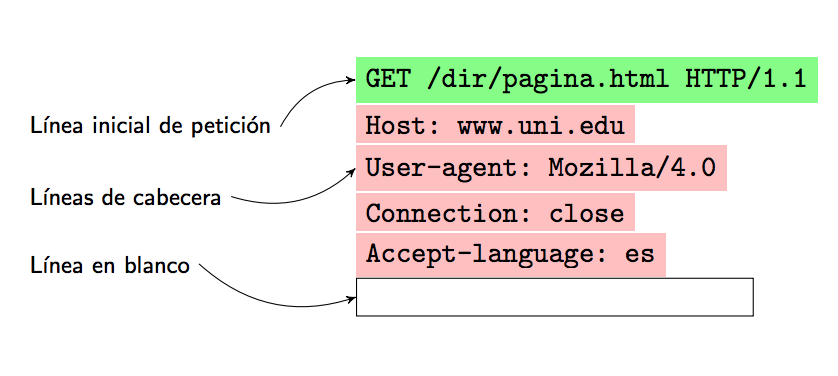
\includegraphics[width=1\linewidth]{chapters/images/peticionhttp.png}
\caption{Ejemplo petición HTTP\\ Cliente a Servidor}
\label{fig:figura1}
\end{minipage}
\hspace{0.5cm}
\begin{minipage}[b]{0.5\linewidth}
\centering
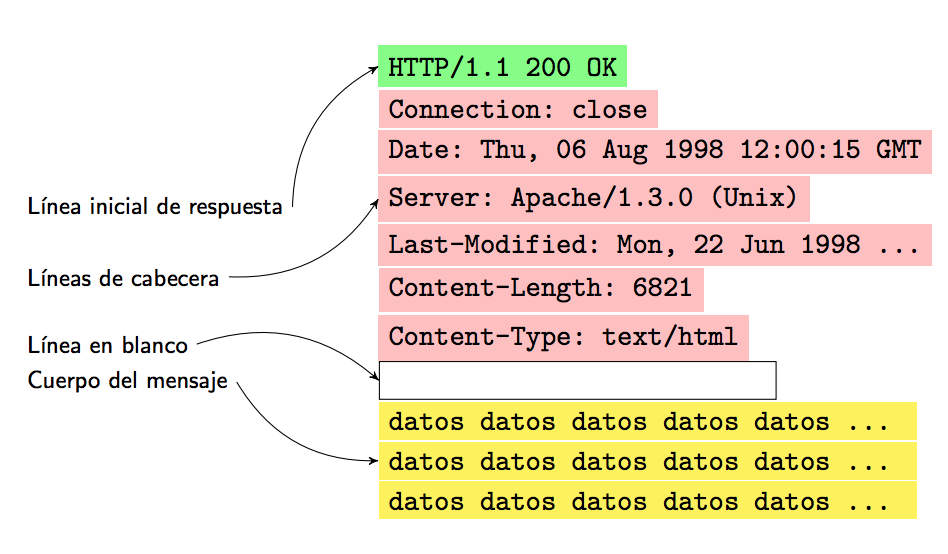
\includegraphics[width=1\linewidth]{chapters/images/respuestahttp.png}
\caption{Ejemplo respuesta HTTP\\ Servidor a Cliente}
\label{fig:figura2}
\end{minipage}
\end{figure}
\begin{figure}[h]
    \centering
    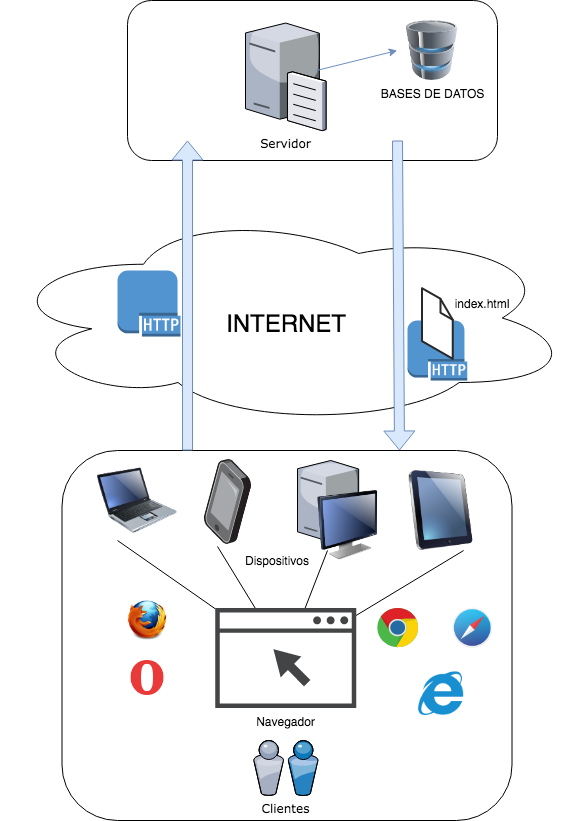
\includegraphics[width=0.5\columnwidth]{chapters/images/web.png}
    \caption{Ejemplo de una comunicación cliente/servidor a través de HTTP}
    \label{fig:httpprotocol}
\end{figure}

Las dos capas que forman una aplicación web son independientes entre sí, pero intercambian información a través del navegador con mensajes HTTP. La tecnologías del  lado cliente (frontend) se encargan de  interactuar con el usuario, visualizar el contenido y establecer la comunicación con el servidor donde el navegador actúa como interprete,  mientras que las tecnologías del lado servidor (backend) se encargan de la administración del sitio web, usando bases de datos y gestores de contenidos.

Una de las principales ventajas de usar tecnologías web es que las aplicaciones creadas son multiplataforma y multidispositivo, funcionan tanto en ordenadores, móviles, tablets, como en distintos sistemas operativos. Otra ventaja es que no tenemos que instalar nada solo necesitamos el navegador y además la actualización del contenido es inmediata. El principal inconveniente es su dependecia de Internet pero con los últimos avances tecnológicos el Wifi, la fibra óptica y el 5G han permitido que  mayoría de personas del mundo podamos acceder desde cualquier lugar y este no sea un gran inconveniente.


\subsection{Tecnologías Web lado cliente}
Las tecnologías web del lado cliente o frontend  permiten la interacción del usuario con la página web que corre en el navegador del usuario. Para ello se usan estas tres tecnologías:

\begin{itemize}
  \item HTML5: es un lenguaje de marcado de los contenidos de un sitio web, se usa para asignar la funcion de cada elemento. Es el esqueleto de la web.
  \item JavaScript: es un lenguaje de programación interpetado que se encarga del comportamiento de una página web y de su interactividad con el usuario.
  \item CSS3: es un lenguaje de hojas de estilo creado para controlar la presentacion de la página: colores, tipo de letra, tamaños, animaciones, colocación de los elementos...
\end{itemize}

Entraremos en más detalle en el capítulo de Herramientas.


\subsection{Tecnologías Web lado servidor}
Las tecnologías web del lado servidor o backend son las que permiten gestionar y servir las páginas web y acceder a bases de datos, en este caso las tecnologías son más flexibles y vamos a nombrar cuatro de las más utilizadas:

\begin{itemize}
    \item Python Django: es una estructura base 'framework' de alto nivel que fomenta el desarrollo rápido con un diseño limpio y práctico destaca por su arquitectura basada en  modelo-vista-controlador y el uso de plantillas (templates). De esta forma puedes centrarte en crear tu aplicacion web sin grandes complicaciones. Es gratis y de código abierto. Un ejemplo de apliación web que utiliza Django es Instagram.  \footnote{https://instagram-engineering.com/web-service-efficiency-at-instagram-with-python-4976d078e366} y Kibotics \footnote{https://kibotics.org}
    \item Node.js: es un entorno de ejecución para JavaScript orientado a eventos síncornos, construido con el motor de JavaScript V8 de Chrome. Diseñado para aplicaciones web escalables. De esta forma el cliente y el sevidor pueden crearse con el mismo lenguaje de programación. Netflix, Paypal o LinkedIn usan esta tecnología para sus servidores. 
    \item webRTC: es un framework que permite las comunicaciones en tiempo real en el navegador. Incluye componentes fundamentales para las comuniaciones de alta calidad en la web. El servidor puede acceder a los componentes de audio y video a través de una API de JavaScript y permite una fácil implementación de la aplicacion chat de voz o video . Podemos destacar aplicaciones como Google Meets o Discord.
    \item PHP: es un lenguaje de scripting de uso general popular que es especialmente adecuado para el desarrollo web. Rápido, flexible y pragmático, gracias a su capacidad de creación de webs dinámicas desde blogs hasta los sitios web como Facebook o Wikipedia.

\end{itemize}


%%%%%%%%%%%%%%%%%%%%%%%%%%%%%%%%%%%%%%%%%%%%%%%%%%%%%%%%%%%%%%%%%%%%%%%%%%%%%%%%%%%%%%%%%%%%%%%%%%%%%%%%%%%%%%%%
\section{Gamificación} \label{gamificacion}
 El término 'Gamificación' o ludificación se emplea para referirse al aprendizaje a través de juegos en el entorno educativo y profesional, los juegos se utilizan para fomentar el aprendizaje de programación y mejorar los conocimientos y habilidades de los alumnos de una forma más dinámica y divertida. La Gamificación facilita la interiorización de los conocimientos, generando una respuesta positiva al usuario por cumplir con un objetivo.
 

\subsection{Importancia de los juegos y multimedia en el aprendizaje} 
La multimedia cada vez está más interiorizada en las aulas y va más allá de las diapositivas. La pandemia vivida en este último año ha impulsado el uso de apliaciones web para dar clase usando plataformas de video conferencia, muchos profesores han optado por estas plataformas y otros han grabado y compartido sus propios videos, de esta forma los estudiantes pueden pararlo y verlo las veces que quieran e interiorizar mejor los conocimientos.\\ Un gran problema existente es que a veces se pide en el aula conocimientos que no se dan, es por ello que se acude a Internet en busca de tutoriales. Un ejemplo es Youtube está lleno de ellos, en los que puedes aprender un monton de cosas y es una buena forma de aprender gracias al contenido multimedia que ofrece. El problema es que a veces los usuarios son demasiado jóvenes y no tienen pensamiento crítico algo muy importante y necesario en Internet.
\\
En los últimos años se están incorporando juegos de encuestas en las aulas como la apliación Kahoot! y  aprendizaje a través de videos y diapositivas más animadas.

*BUSCAR ALGUN ARTICULO*



\subsection{Robótica educativa} 
La Robótica educativa es una disciplina de aprendizaje multidisciplinar. Ayuda a desarrollar competencias y habilidades como: la innovación y espíritu emprendedor, la resolución de problemas y lógica, la toma de decisiones, conocimientos de herramientas relacionadas con las tecnologías digitales, el pensamiento crítico, creatividad, el trabajo colaborativo y cooperativo, la flexibilidad y adaptabilidad al trabajo. *poner referencia.
\\
Ante la falta de estudiantes en carreras técnicas en la actualidad, la robótica educativa puede ofrecer una gran motivación a los alumnos de las primeras etapas de educación: Primaria, ESO y Bachillerato, para fomentar la creatividad y la curiosidad al mostrar la ciencia y la tecnología de una forma más dinámica y divertida, incrementan sus habilidades a la vez que sus conocimientos desde los fundamentos STEM (Science, Technology, Engineering and Mathematics).

Gracias a las tecnologías web muchas aplicaciones ofrecen cursos de robótica para todos los niveles educativos, muchos ayuntamientos estan comprando cursos y materiales y para facilitar a los más pequeños su introducción al mundo de la robótica a través de clases extraescolares. En secuandaria, se estan introduciendo poco a poco en las asignaturas de tecnología el uso de lenguajes de programación en el que destaca por encima de todos el lenguaje Scratch.

Scratch es un lenguaje de programación visual basado en bloques, creado y  mantenido por Lifelong Kindergarten group en el MIT Media Lab.*referencia Scratch además es una comunidad en línea donde los niños pueden programar y compartir medios interactivos como historias, juegos y animaciones con gente de todo el mundo. Los más pequeños pueden aprenden a pensar creativamente, trabajar en colaboración y razonar sistemáticamente. Scratch posee un lenguaje de iniciación llamado Scratch Jr pensando para niños de 5 a 7 años siendo aún más sencillo, aunque Scratch está pensado para todas las edades. Actualmente se puede utilizar desde cualquier dispositivo al ultilizar tecnologías web.


El mejor ejemplo de una plataforma educativa es Kibotics, plataforma en la que esta basada este trabajo. 
Kibotics es un entorno web para docencia en robótica y programación (STEM). Enseña de manera atractiva conceptos básicos de tecnología (informática, electrónica, ...) e inicia a niños y adolescentes en robótica y programación de robots. Sigue un enfoque práctico, de aprender haciendo. Ayuda a estructurar el pensamiento, a organizar las acciones en pasos para resolver un problema y a formar espíritu analítico. *REFERENCIA
\\
Esta plataforma ofrece cursos de robótica en Scratch y Python. Basado en tecnologías web como Django y el simulador Websim apoyado en  A-Frame para representar los escenarios de los ejercicios. En el capítulo de Herramientras se matizará un poco más estas tecnologías. 

Actualmente cuentan con ejercicios que fomentan el aprendizaje como el cuadrado, busca objeto, choca-gira, sigue-lineas. A lo largo de este trabajo veremos como se introduce la Gamificación en la plataforma.


\subsection{Campeonatos de robótica educativa existentes}

El aprendizaje de la robótica ha ido más allá y actualmente existen competiciones a nivel Nacional e Internacional estas son algunas de ellas:
*poner algo más
\begin{itemize}
    \item RoboCup Junior
    \item RoboCampeones
    \item Eurobot Junior
    \item First Lego league
    \item Torneo Nacional VEX Robotics IQ
\end{itemize}
